
% this file is called up by thesis.tex
% content in this file will be fed into the main document

%: ----------------------- introduction file header -----------------------


\chapter{Ap\'endice}
\label{cha:apendice}

\section{Igualdades trigonom\'etricas}

Dedicamos esta secci\'on a recopilar las f\'ormulas de trigonometr\'ia hiperb\'olica utilizadas durante \'este trabajo. Comenzamos con las f\'ormulas para seno y coseno hperb\'olicos:

 \begin{eqnarray}
 cosh(x \pm y)= coshxcoshy \pm sinhxsinhy \\
 sinh(x \pm y)=sinhxcoshy \pm coshxsinhy \\
 cosh2x=cosh^{2}x+sinh^{2}x=2cosh^{2}x-1 \\
 sinh2x = 2sinhx\cdot coshx
 \end{eqnarray}

 Para tri\'angulos hiperb\'olicos tenemos lo siguiente: \\

 Sea $\vartriangle (A,B,C)$ un tri\'angulo con lados $A, B $ y $ C$. Y sean sus correspondientes \'angulos opuestos $\alpha,\beta$ y $\gamma$ entonces, si $\gamma$ es un angulo recto tenemos; \\

 Ley de los cosenos hiperb\'olicos
 \begin{equation}
 cosh C = cosh A\cdot cosh B
 \end{equation}

 Ley de los senos hiperb\'olicos
 \begin{equation}
 sinhB = sinhA \cdot tan \beta
 \end{equation}

 Tambi\'en
 \begin{eqnarray}
 cosh A \cdot sin \beta = cos \alpha  \\
 coshB \cdot sin \alpha= cos \beta
 \end{eqnarray}

 Para tri\'angulos arbitrarios se tiene; \\

 Ley de los cosenos hiperb\'olicos
 \begin{equation}
 coshC=coshA \cdot coshB - sinhA\cdot sinhB\cdot cos \gamma
 \end{equation}

Ley de los senos hiperb\'olicos
\begin{equation}
\frac{sinhA}{sin \alpha} =\frac{sinhB}{sin \beta}= \frac{sinhC}{sin \gamma}
\end{equation}

Para un cuadrilatero con tres \'angulos rectos como en la figura \ref{apendice1}, donde $\Phi$ no es recto, se tiene:

\begin{eqnarray}
sinhD\cdot sinhA =cos \Phi \\
cosh D = cosh B \cdot sin \Phi \\
coshA=coshC\cdot sin \Phi
\end{eqnarray}

\begin{figure}[h]
  \centering
  % Requires \usepackage{graphicx}
  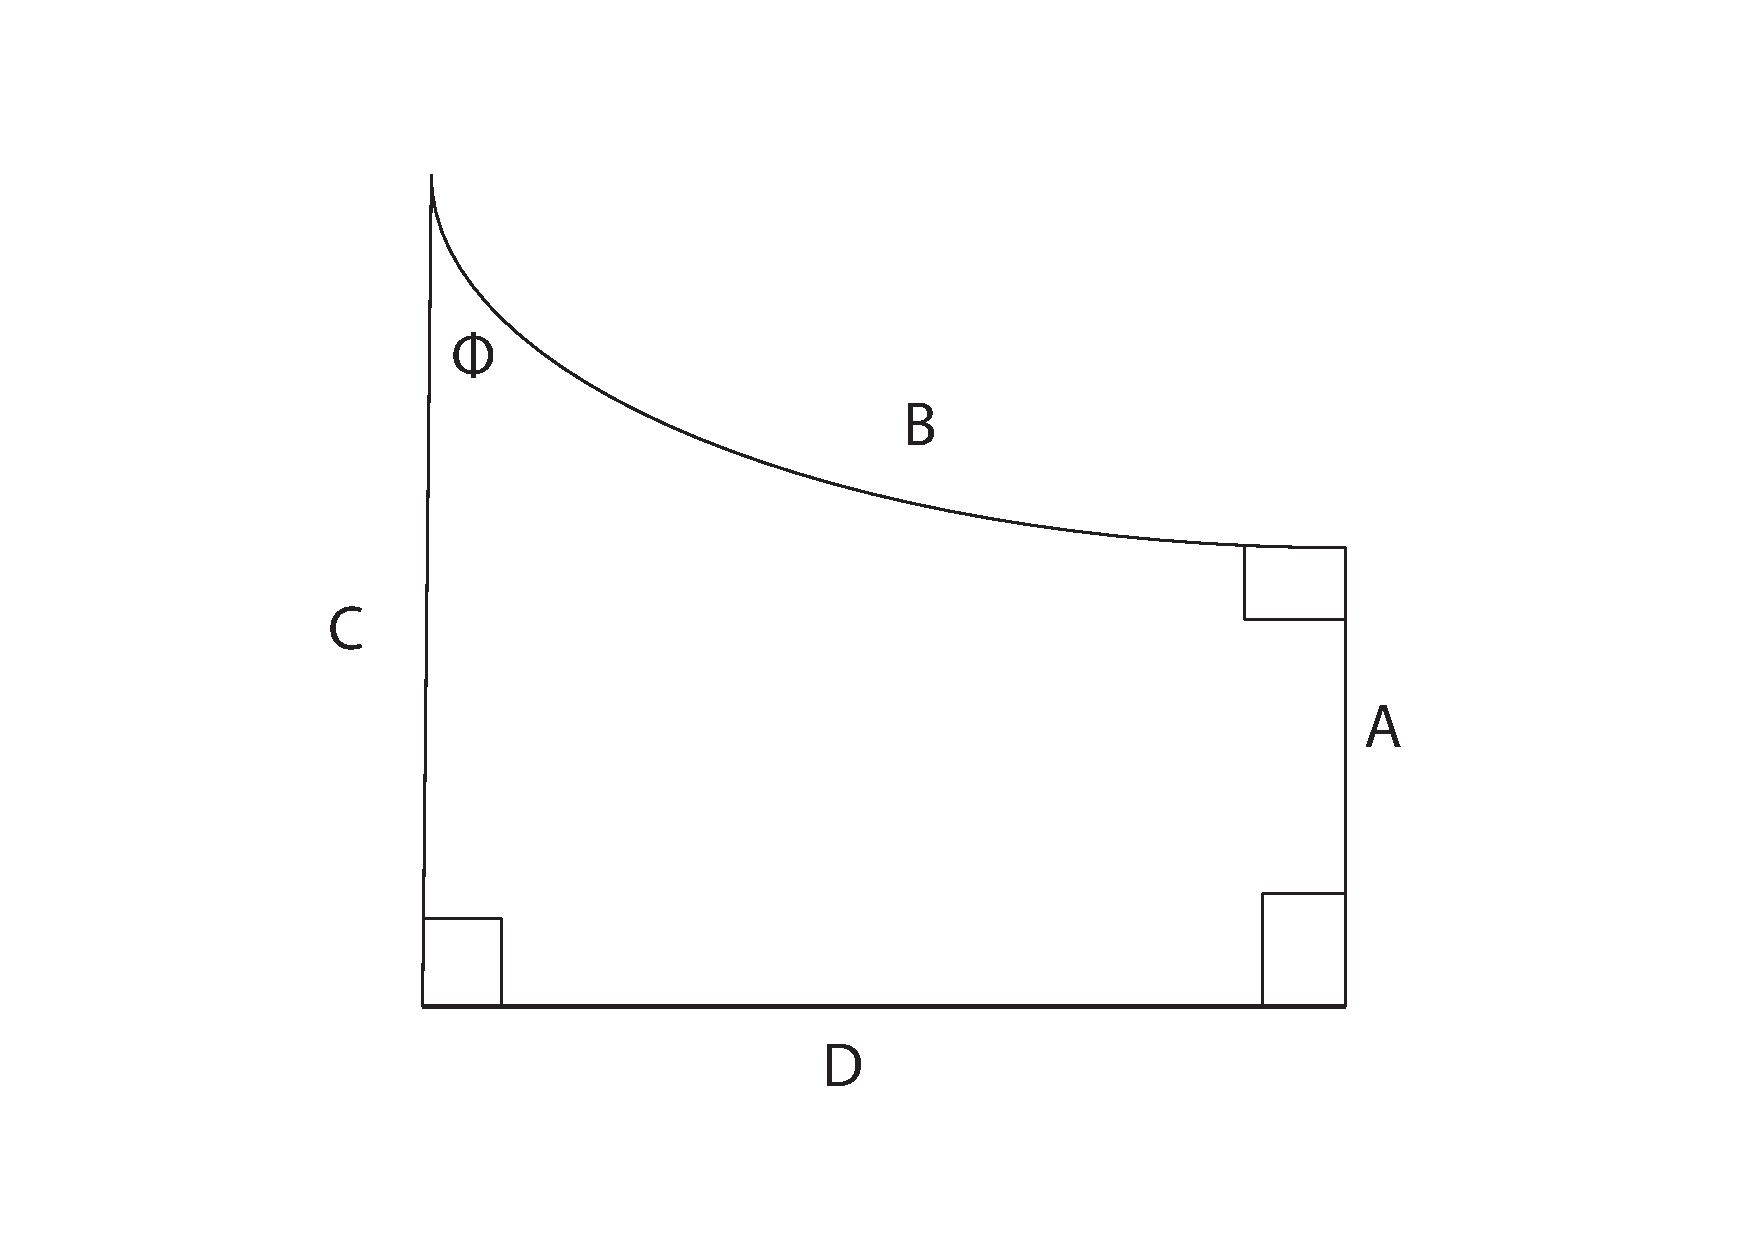
\includegraphics[width=10cm]{apendice1}\\
  \caption{Cuadrilatero con 3 \'angulos rectos}\label{apendice1}
\end{figure}

En un tri\'angulo $\vartriangle (A,B,C)$ hay una relaci\'on entre $\gamma$ y la longitud de $C$

$$coshC > coshA\cdot coshB \ si \ \gamma < \frac{\pi}{2}$$
$$ coshC = coshA \cdot coshB \ si  \ \gamma= \frac{\pi}{2}$$
$$ coshC < coshA \cdot coshB \ si \ \gamma > \frac{\pi}{2}$$

Por \'ultimo tenemos un resultado para pentagonos con 4 \'angulos rectos.

Sea $P$ un pent\'agono como en la figura \ref{apendice2}, donde $h,D$ son medidas de los lados  y $H$ la medida de la perpendicular del v\'ertice al lado $s$ y denotamos por $s$ tambi\'en a su medida.

\begin{figure}[h]
  \centering
  % Requires \usepackage{graphicx}
  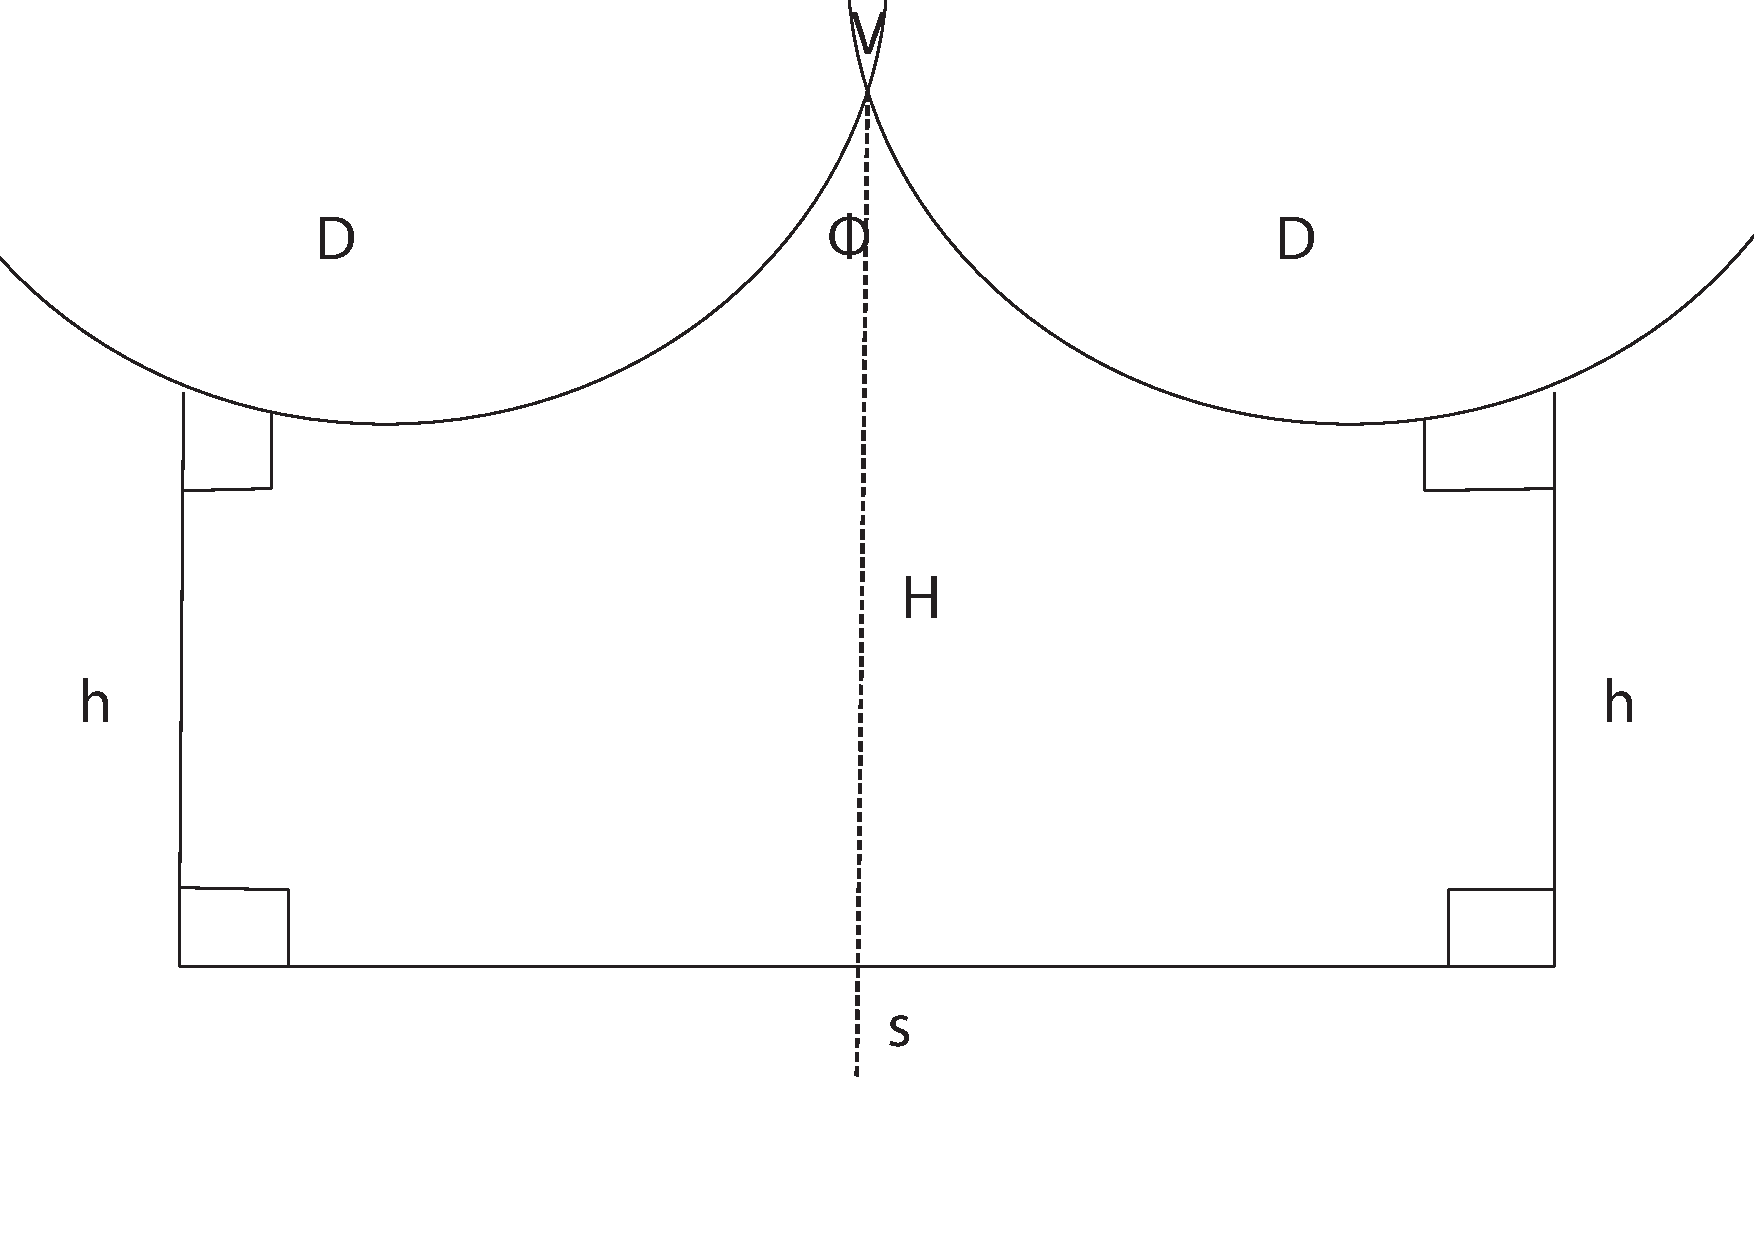
\includegraphics[width=10cm]{apendice2}\\
  \caption{Pent\'agono con 4 \'angulos rectos}\label{apendice2}
\end{figure}

Las siguientes condiciones se cumplen 

\begin{eqnarray}
sinh \cdot sinh \frac{s}{2}= cos (\frac{\Phi}{2}) \\
cosh=coshH \cdot sin (\frac{\Phi}{2}) \\
cosh \frac{s}{2} = coshD \cdot sin (\frac{\Phi}{2})
\end{eqnarray}


\section{Teorema de Cauchy}


\section{Mapeo y principio de reflexi\'on de Schwarz}

Si consideramos la ecuaci\'on diferencial hipergeom\'etrica 

$$ x(1-x)u''+(c-(a+b+1)x)u'-abu=0$$

Cualesquiera dos soluciones linealmente independientes $u_{1},u_{2}$ definen un mapeo

$$s: \mathbb{C}-\lbrace 0,1 \rbrace \ni x \mapsto u_{1}(x):u_{2}(x) \in \widehat{\mathbb{C}} $$

Al que llamamos el mapeo de Schwarz. El teorema fundamental de Cauchy nos asegura que dos soluciones linealmente independientes no son simultaneamente cero en $\mathbb{C}-\lbrace 0,1 \rbrace $. Para un estudio mas profundo del mapeo de Scwarz se remite al lector a \cite{geometricstudy}.

EL principio de reflexi\'on de Schwarz se enuncia de la siguiente manera:

\begin{prop}
Sea $f$ una funci\'on holomorfa en un dominio $D$ cuya frontera contiene un intervalo real $(a,b)$. Supongamos que $f$ se puede extender a una funci\'on continua en $D \cup (a,b)$ y es real valuada en el intervalo $(a,b)$. Extendiendo $f$ por

$$f(x):= \bar{f(\bar{x})}, \ x\in \bar{D}:= \lbrace \bar{\xi} | \xi \in D \rbrace $$

A la imagen reflejada $\bar{D}$ de $D$. Entonces, la extensi\'on de $f$ es holomorfa en $D \cup (a,b) \cup \bar{D}$, y su imagen es la uni\'on de $f(D)$, su imagen reflejada $\bar{f(D)}$ y el intervalo $f((a,b))$ que comparten como parte de su frontera. 
\end{prop}

\begin{figure}[h]
  \centering
  % Requires \usepackage{graphicx}
  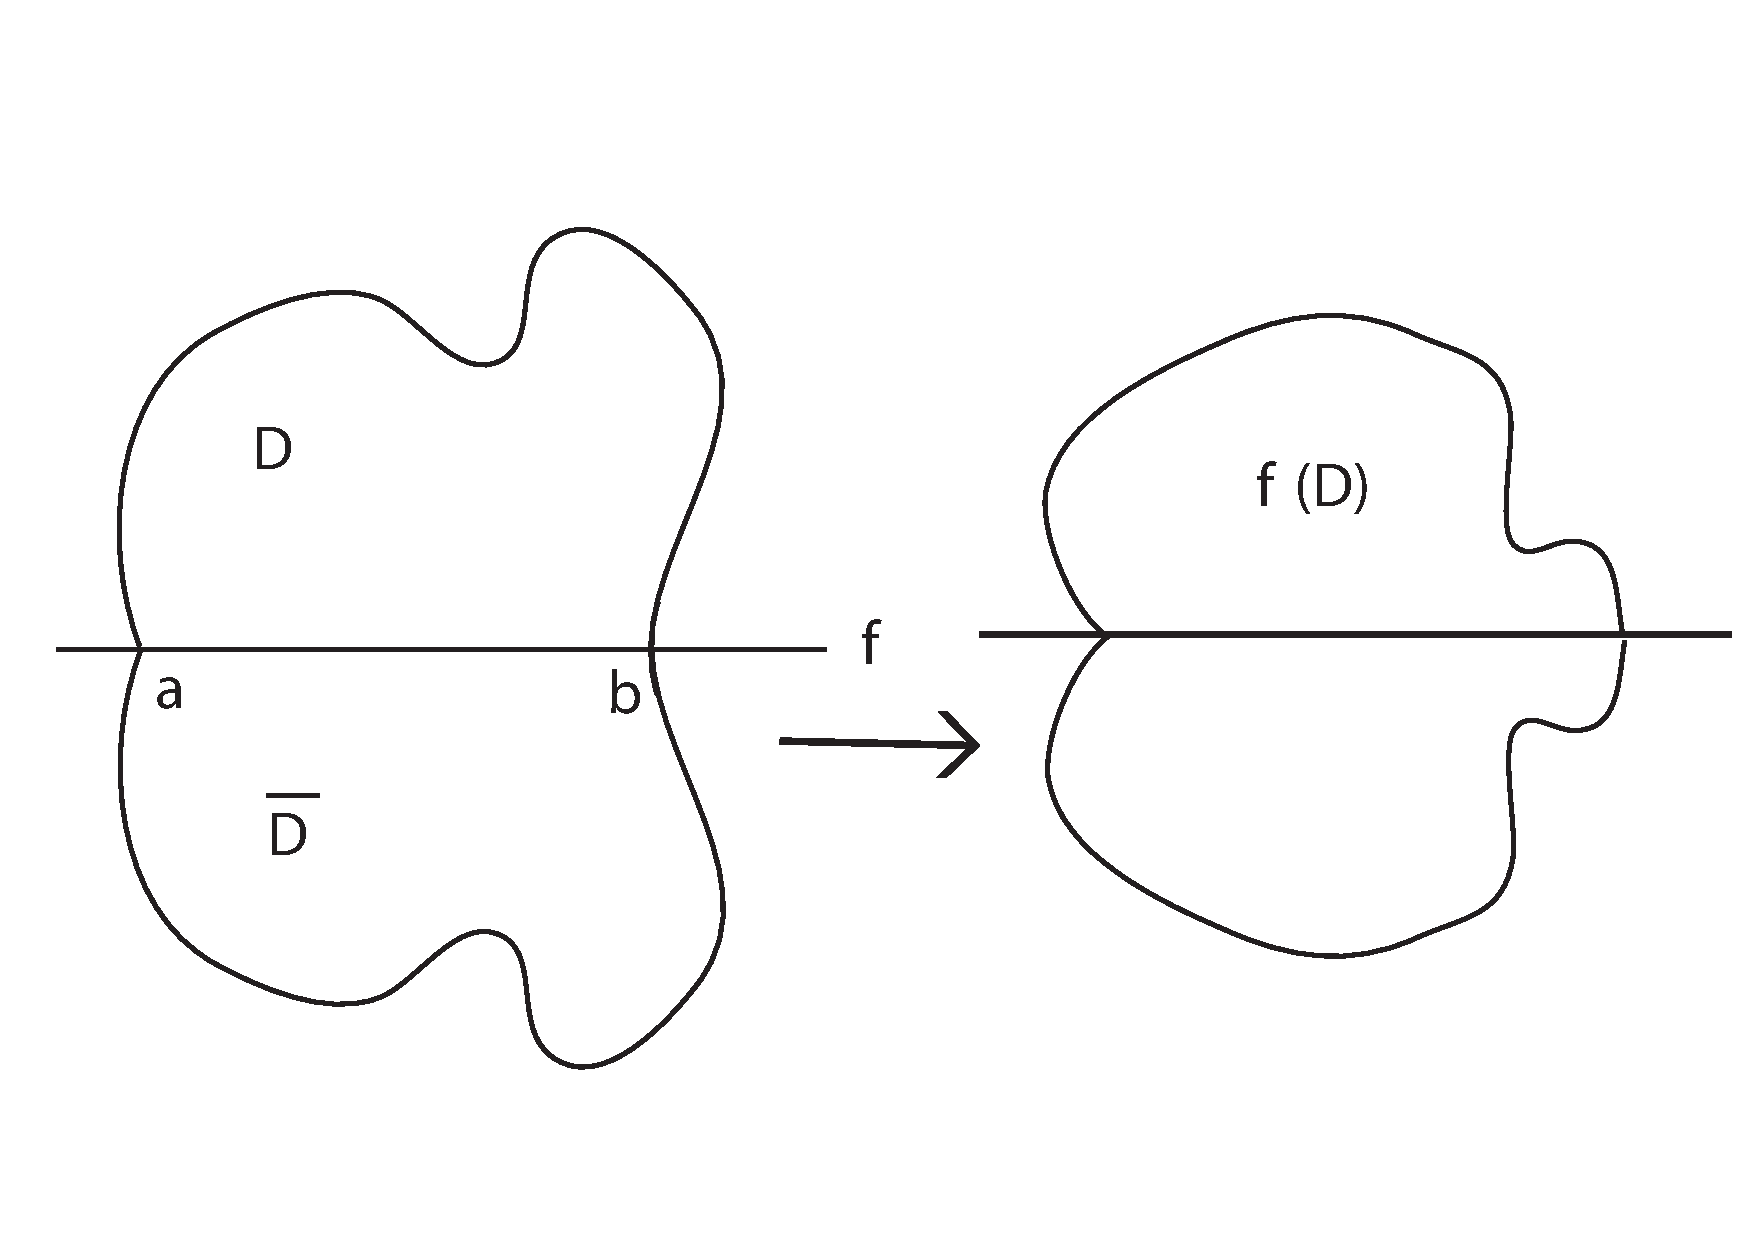
\includegraphics[width=10cm]{apendice3}\\
  \caption{Principio de reflexi\'on de Schwarz}\label{apendice3}
\end{figure}



% the code below specifies where the figures are stored
\ifpdf
    \graphicspath{{5_conclusion/figures/PNG/}{5_conclusion/figures/PDF/}{5_conclusion/figures/}}
\else
    \graphicspath{{5_conclusion/figures/EPS/}{5_conclusion/figures/}}
\fi


%-------------------------------------------------------------------------


% ----------------------------------------------------------------------


